\section{Transformation to Abstract Syntax Graph}

We describe here the transformation of user-facing ESMoL language objects and
relations to a more compact set of relations that simplify generation of design
artifacts from the model.  The most direct example of such a semantic assumption
is the single-message abstraction.  Data transfers between the functional code
and the message fields must be compatible. We enforce that both by constraint
checking, and by the assumption of a single semantic message object for all
participants in the data interchange.  The Signal object (not shown) in the
abstract graph represents the transfer of a single datum to or from the message.

The transformations shown capture different forms of the
single-message transformation.  This is not a complete description of the
entire first stage transformation, but provides a representative subset for
illustration. The actual transformation is implemented in C++ using the UDM
modeling API\cite{mic:udm}.

In the formal descriptions below, $Obj_{Type}$ is the set of objects of type $Type$, and
$obj_{Type}$ is an instance from that set.  We also
use two functions $id: Obj_{Type} \rightarrow \mathbf{Z}^{+}$ for a unique
identifier of an object, and $parent: Obj_{Type1} \rightarrow Obj_{Type2}$ to
find the parent (defined by a containment relation in the model of an object).

\subsection{Acquisition: From the Environment to Data}

In ESMoL\_Abstract \emph{Acquisition} objects relate all of the different model entities (and
therefore, their design parameters) that participate in the collection of data
from an input device such as an analog to digital converter or serial link.

\begin{table}[ht]
\centering

\begin{tabular}[width=\columnwidth]{ | l | l | }
 \hline
 \textbf{Specified ESMoL Relation Sets} & \textbf{Semantic
Construct} \\
 \hline \hline
                                                                        & \\
 $CA_{id_N} = \{ (obj_{Node}, obj_{CompInst} ) \, |$                    & \\
 \hspace{1.7cm} $ id(obj_{Node}) = id_N \} $                            & \\
                                                                        & \\
 $AC_{id_{Ch}} = \{ (obj_{IChan}, obj_{MsgInst} ) \, |$                 & 
$ Acq = \{(obj_{MsgInst}, obj_{CompInst}, $  \\
 \hspace{1.6cm} $id(obj_{IChan}) = id_{Ch} \} $                         & 
\hspace{1.3cm} $obj_{N}, obj_{Ch}) \, |$ \\
                                                                        &  
\hspace{0.8cm} $(obj_{N}, obj_{CompInst}) \in CA_{id_N}$ \\
 $NC_{id_N} = \{ (obj_{Node}, obj_{IChan}) \, | $                       & 
\hspace{0.5cm} $ \wedge \, (obj_{Ch}, obj_{MsgInst}) \in AC_{id_{Ch}}$ \\
 \hspace{1.35cm} $id(obj_{Node}) = id_N $                                &
\hspace{0.5cm} $ \wedge \, (obj_{N}, obj_{IChan}) \in NC_{id_N}$ \\ 
 \hspace{1cm} $ \wedge \, parent(obj_{IChan} ) = obj_{Node} \}$       &
\hspace{0.5cm} $ \wedge \, (obj_{CompInst}, obj_{MsgInst}) \in CC $ \\
                                                                        & \\
 $CC = \{ (obj_{CompInst}, obj_{MsgInst} ) \, | $                       & \\
 \hspace{0.7cm} $parent(obj_{MsgInst} ) = obj_{CompInst} \}$            & \\ 
                                                                        & \\
 \hline
\end{tabular}
	\caption{Depiction of the transformation step that takes ESMoL
relation objects on the left, and produces a single relation for each
collection representing a data acquisition specfication.}
	\label{tab:acquisition}
\end{table}

The ESMoL relations shown in table \ref{tab:acquisition} are as follows:

\begin{itemize}
 \item $CA$ {\bf ComponentAssignment}: (the dashed connection shown in 
Fig. \ref{fig:qr_hw_mapping}) assigns a task to run on a particular 
processor ($id_N$).
 \item $AC$ {\bf AcquisitionConnection}: (the directed connection from 
processor ports to component message ports) assigns a hardware input peripheral
(modeled as an object of type $IChan$) to a message structure compatible with the
component.
 \item $NC$: Containment relationship of the channel object (port) in the Node object.
 \item $CC$: Containment of the message instance object (port) in the component instance object.
\end{itemize}

The metalanguage for ESMoL\_Abstract captures the structural
semantic reductions shown in table \ref{tab:acquisition} in a compact form (see
Fig. \ref{fig:acq_meta}), so that all of the consumers of the input data get the
same consistent structural view of the model.  The modeling tools provide a
programming interface for traversing, reading, and editing the models.

\begin{figure}[htb]
\centering
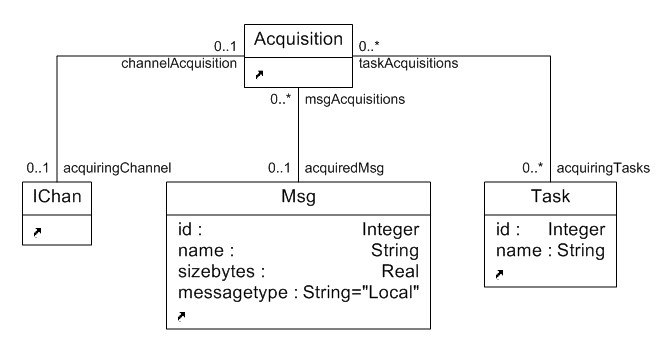
\includegraphics[width=0.9\columnwidth]{figures/acquisition.png}
    \caption{Acquistion relation in ESMoL Abstract. Acquistion represents
data arriving from the environment. The abstract syntax graph
model collects all of the information scattered over multiple relations in the
user-facing language, and stores them in one relation for consumption by the
synthesis interpreters. Each of these communication relations supports one
sender and multiple receivers. }
    \label{fig:acq_meta}
\end{figure}

The collected relations are more easily processed by the synthesis interpreters,
as they avoid extra traversals to gather the other relations.  For acquisition 
and actuation (below), data transfers are timed in the current version of the 
execution environment.  Work is currently underway to fully support event-driven 
messaging and activation of sporadic tasks.

\subsection{Actuation: From Data Back to the Environment}

% \begin{table*}[h]
% \centering
% 
% \begin{tabular}[width=\columnwidth]{ | l | l | }
%  \hline
%  \textbf{Specified ESMoL Relation Sets} & \textbf{Semantic
% Construct} \\
%  \hline \hline
%                                                                         & \\
%  $CA_{id_N} = \{ (obj_{Node}, obj_{CompInst} ) \, |$                    & \\
%  \hspace{1.7cm} $ id(obj_{Node}) = id_N \} $                            & \\
%                                                                         & \\
%  $AC_{id_{Ch}} = \{ (obj_{OChan}, obj_{MsgInst} ) \, |$                 & 
% $ Act = \{(obj_{MsgInst}, obj_{CompInst}, $  \\
%  \hspace{1.6cm} $id(obj_{OChan}) = id_{Ch} \} $                         & 
% \hspace{1.3cm} $obj_{N}, obj_{Ch}) \, |$ \\
%                                                                         &  
% \hspace{0.8cm} $(obj_{N}, obj_{CompInst}) \in CA_{id_N}$ \\
%  $NC_{id_N} = \{ (obj_{Node}, obj_{OChan}) \, | $                       & 
% \hspace{0.5cm} $ \wedge \, (obj_{Ch}, obj_{MsgInst}) \in AC_{id_{Ch}}$ \\
%  \hspace{1.35cm} $id(obj_{Node}) = id_N $                               &
% \hspace{0.5cm} $ \wedge \, (obj_{N}, obj_{OChan}) \in NC_{id_N}$ \\ 
%  \hspace{1cm} $ \wedge \, parent(obj_{OChan} ) = obj_{Node} \}$         &
% \hspace{0.5cm} $ \wedge \, (obj_{CompInst}, obj_{MsgInst}) \in CC $ \\
%                                                                         & \\
%  $CC = \{ (obj_{CompInst}, obj_{MsgInst} ) \, | $                       & \\
%  \hspace{0.7cm} $parent(obj_{MsgInst} ) = obj_{CompInst} \}$            & \\ 
%                                                                         & \\
%  \hline
% \end{tabular}
% 	\caption{Actuation relation transformation.}
% 	\label{tab:actuation}
% \end{table*}

\begin{figure}[h]
\centering
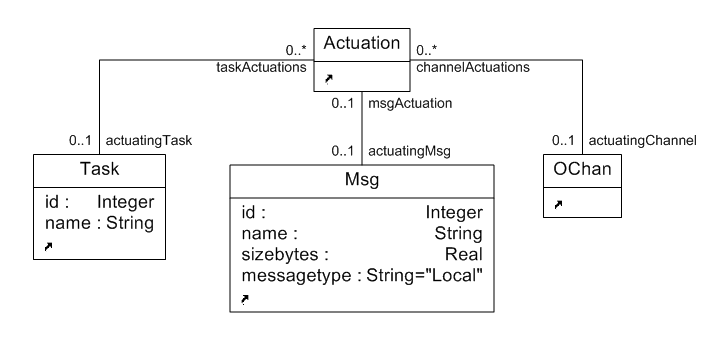
\includegraphics[width=0.9\columnwidth]{figures/actuation.png}
    \caption{Actuation relation in ESMoL Abstract. Actuation represents the
flow of data back into the environment.}
    \label{fig:act_meta}
\end{figure}

The transformation to an Actuation object is nearly identical to that of the 
Acquisition transformation, but the data direction, cardinalities, and types 
involved are different.  Fig. \ref{fig:acq_meta} shows the resulting construct in
the abstract language.

\subsection{Local Dependencies: Data Movement within Nodes}

\begin{table*}[h]
\centering

\begin{tabular}[width=\columnwidth]{ | l | l | }
 \hline
 \textbf{Specified ESMoL Relation Sets} & \textbf{Semantic
Construct} \\
 \hline \hline
                                                                        & \\
 $CA_{id_N} = \{ (obj_{Node}, obj_{CompInst} ) \, |$                    & \\
 \hspace{1.7cm} $ id(obj_{Node}) = id_N \} $                            & \\
                                                                        & 
$ Locals = \{(obj_{MsgInst1}, obj_{CompInst1}, $  \\
 $LD_{id_1} = \{ (obj_{MsgInst1}, obj_{MsgInst} ) \, |$             & 
\hspace{0.7cm} $obj_{MsgInst2}, obj_{CompInst2}, obj_{N}) \, |$ \\
 \hspace{1.9cm} $id(obj_{MsgInst1}) = id_1 \} $                & 
\hspace{0.5cm} $(obj_{N}, obj_{CompInst1}) \in CA_{id_N}$ \\
                                                                        &  
\hspace{0.2cm} $\wedge \, (obj_{N}, obj_{CompInst2}) \in CA_{id_N}$ \\
 $LD_{TC} = \{ (obj_{MsgInstj}, obj_{MsgInstj+1}) |  $ & 
\hspace{0.2cm} $ \wedge \, (obj_{MsgInst1}, obj_{MsgInst2}) \in LD_{TC}$
\\
 \hspace{0.3cm} $ in \, the \, sequence  $ &
\hspace{0.15cm} $ \wedge \, (obj_{CompInst}, obj_{MsgInst}) \in CC $ \\
 \hspace{0.4cm} $  ( (obj_{MsgInst1}, obj_{MsgInst2}) \in LD_{id_1}, $ &
\\
 \hspace{0.4cm} $ (obj_{MsgInst2}, obj_{MsgInst3}) \in LD_{id_2}, $ & \\
 \hspace{0.7cm} \dots & \\
 \hspace{0.4cm} $ (obj_{MsgInstj}, obj_{MsgInstj+1}) \in LD_{id_j} ) \} $
& \\
 & \\
 $CC = \{ (obj_{CompInst}, obj_{MsgInst} ) \, | $  & \\
 \hspace{0.3cm} $parent(obj_{MsgInst} ) = obj_{CompInst} \}$ & \\
 & \\
 \hline
\end{tabular}
	\caption{Local (processor-local) data dependency relation.}
	\label{tab:localdeps}
\end{table*}

Local dependencies represent not only direct data dependencies between nodes on
a particular processor, but also implied dependencies through remote data
transfer chains starting and ending on the same processor.   This is modeled as
the set $LD_{TC}$ of all pairs in the transitive closure of dependencies
starting with the message instance $obj_{MsgInst1}$. The collected set of local
dependencies ( $Locals$ ) intersects this set with those message instances
contained in components on the current processing node (i.e. from the set $CA_{id_N}$).

\begin{figure}
\centering
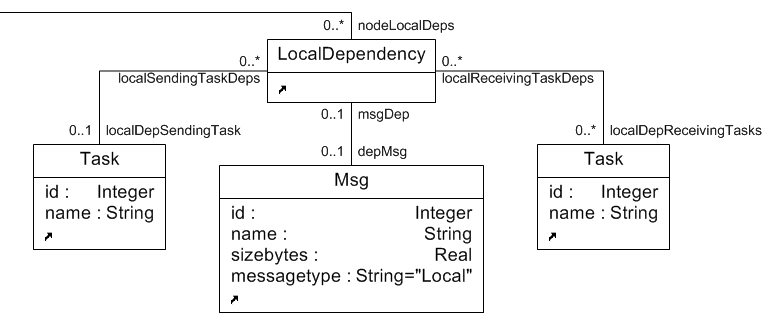
\includegraphics[width=0.9\columnwidth]{figures/localdeps.png}
    \caption{Local dependency relation in ESMoL Abstract. Local data
transfers take place between components on the same processing node.}
    \label{fig:localdep_meta}
\end{figure}

\subsection{ Bus Transfers: Data Movement Between Nodes}

Bus transfers are slightly more complicated, as they involve two or more
endpoints.  Table \ref{tab:transmit} along with Fig.
\ref{fig:trnrcv_meta} show the details. The platform-specific code generators
produce separate files for each processing node (especially as the nodes
may be heterogeneous), so the send and receive relations are modeled separately. Fig. 
\ref{fig:msg_sched} shows an example of the objects and parameters based on our
design example.  The object network is an instance of the abstract language construct
shown in Fig. \ref{fig:trnrcv_meta}.

\begin{table}[h]
\centering

\begin{tabular}[width=\columnwidth]{ | l | l | }
 \hline
 \textbf{Specified ESMoL Relation Sets} & \textbf{Semantic
Construct} \\
 \hline \hline
                                                                        & \\
 $CA_{id_N} = \{ (obj_{Node}, obj_{CompInst} ) \, |$                    & \\
 \hspace{1.7cm} $ id(obj_{Node}) = id_N \} $                            & \\
                                                                        & \\
 $AC_{id_{Ch}} = \{ (obj_{MsgInst}, obj_{BChan} ) \, |$          
   & 
$ Trn = \{(obj_{MsgInst}, obj_{CompInst}, $  \\
 \hspace{1.6cm} $id(obj_{BChan}) = id_{Ch} \} $                         & 
\hspace{1.3cm} $obj_{N}, obj_{Ch}) \, |$ \\
                                                                        &  
\hspace{0.8cm} $(obj_{N}, obj_{CompInst}) \in CA_{id_N}$ \\
 $NC_{id_N} = \{ (obj_{Node}, obj_{BChan}) \, | $                       & 
\hspace{0.5cm} $ \wedge \, (obj_{Ch}, obj_{MsgInst}) \in AC_{id_{Ch}}$ \\
 \hspace{1.35cm} $id(obj_{Node}) = id_N $                               &
\hspace{0.5cm} $ \wedge \, (obj_{N}, obj_{BChan}) \in NC_{id_N}$ \\ 
 \hspace{1cm} $ \wedge \, parent(obj_{BChan} ) = obj_{Node} \}$         &
\hspace{0.5cm} $ \wedge \, (obj_{CompInst}, obj_{MsgInst}) \in CC $ \\
                                                                        & \\
 $CC = \{ (obj_{CompInst}, obj_{MsgInst} ) \, | $                       & \\
 \hspace{0.7cm} $parent(obj_{MsgInst} ) = obj_{CompInst} \}$            & \\ 
                                                                        & \\
 \hline
\end{tabular}
	\caption{Transmit relation in the abstract graph.  This represents the
sender side of a remote data transfer between components. The Receives relation 
has an identical structure, but cardinality is differnt. Each Receives
relation object represents a receiver in a remote data transfer between
components. A single sender may have multiple receivers attached to the same
message.}
	\label{tab:transmit}
\end{table}

% \begin{table}[h]
% \centering
% 
% \begin{tabular}[width=\columnwidth]{ | l | l | }
%  \hline
%  \textbf{Specified ESMoL Relation Sets} & \textbf{Semantic
% Construct} \\
%  \hline \hline
%                                                                         & \\
%  $CA_{id_N} = \{ (obj_{Node}, obj_{CompInst} ) \, |$                    & \\
%  \hspace{1.7cm} $ id(obj_{Node}) = id_N \} $                            & \\
%                                                                         & \\
%  $AC_{id_{Ch}} = \{ (obj_{BChan}, obj_{MsgInst} ) \, |$          
%    & 
% $ Rcv = \{(obj_{MsgInst}, obj_{CompInst}, $  \\
%  \hspace{1.6cm} $id(obj_{BChan}) = id_{Ch} \} $                         & 
% \hspace{1.3cm} $obj_{N}, obj_{Ch}) \, |$ \\
%                                                                         &  
% \hspace{0.8cm} $(obj_{N}, obj_{CompInst}) \in CA_{id_N}$ \\
%  $NC_{id_N} = \{ (obj_{Node}, obj_{BChan}) \, | $                       & 
% \hspace{0.5cm} $ \wedge \, (obj_{Ch}, obj_{MsgInst}) \in AC_{id_{Ch}}$ \\
%  \hspace{1.35cm} $id(obj_{Node}) = id_N $                               &
% \hspace{0.5cm} $ \wedge \, (obj_{N}, obj_{BChan}) \in NC_{id_N}$ \\ 
%  \hspace{1cm} $ \wedge \, parent(obj_{BChan} ) = obj_{Node} \}$         &
% \hspace{0.5cm} $ \wedge \, (obj_{CompInst}, obj_{MsgInst}) \in CC $ \\
%                                                                         & \\
%  $CC = \{ (obj_{CompInst}, obj_{MsgInst} ) \, | $                       & \\
%  \hspace{0.7cm} $parent(obj_{MsgInst} ) = obj_{CompInst} \}$            & \\ 
%                                                                         & \\
%  \hline
% \end{tabular}
% 	\caption{Receive relation in the abstract graph.  Each $Receives$
% relation object represents a receivers in a remote data transfer between
% components. A single sender may have multiple receivers attached to the same
% message.}
% 	\label{tab:receive}
% \end{table}

\begin{figure}
\centering
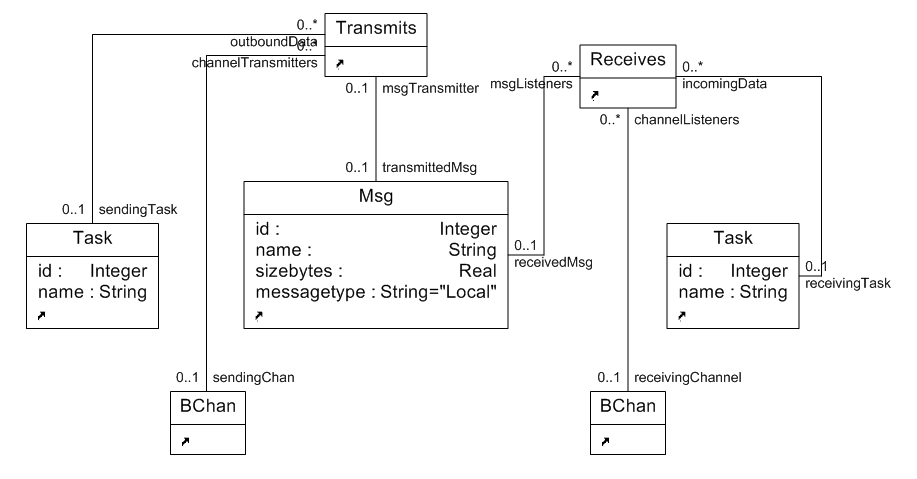
\includegraphics[width=0.9\columnwidth]{figures/tran_rcv.png}
    \caption{Transmit and receive relations in ESMoL Abstract. These
represent the endpoints of data transfers between nodes.}
    \label{fig:trnrcv_meta}
\end{figure}

\begin{figure}
\centering
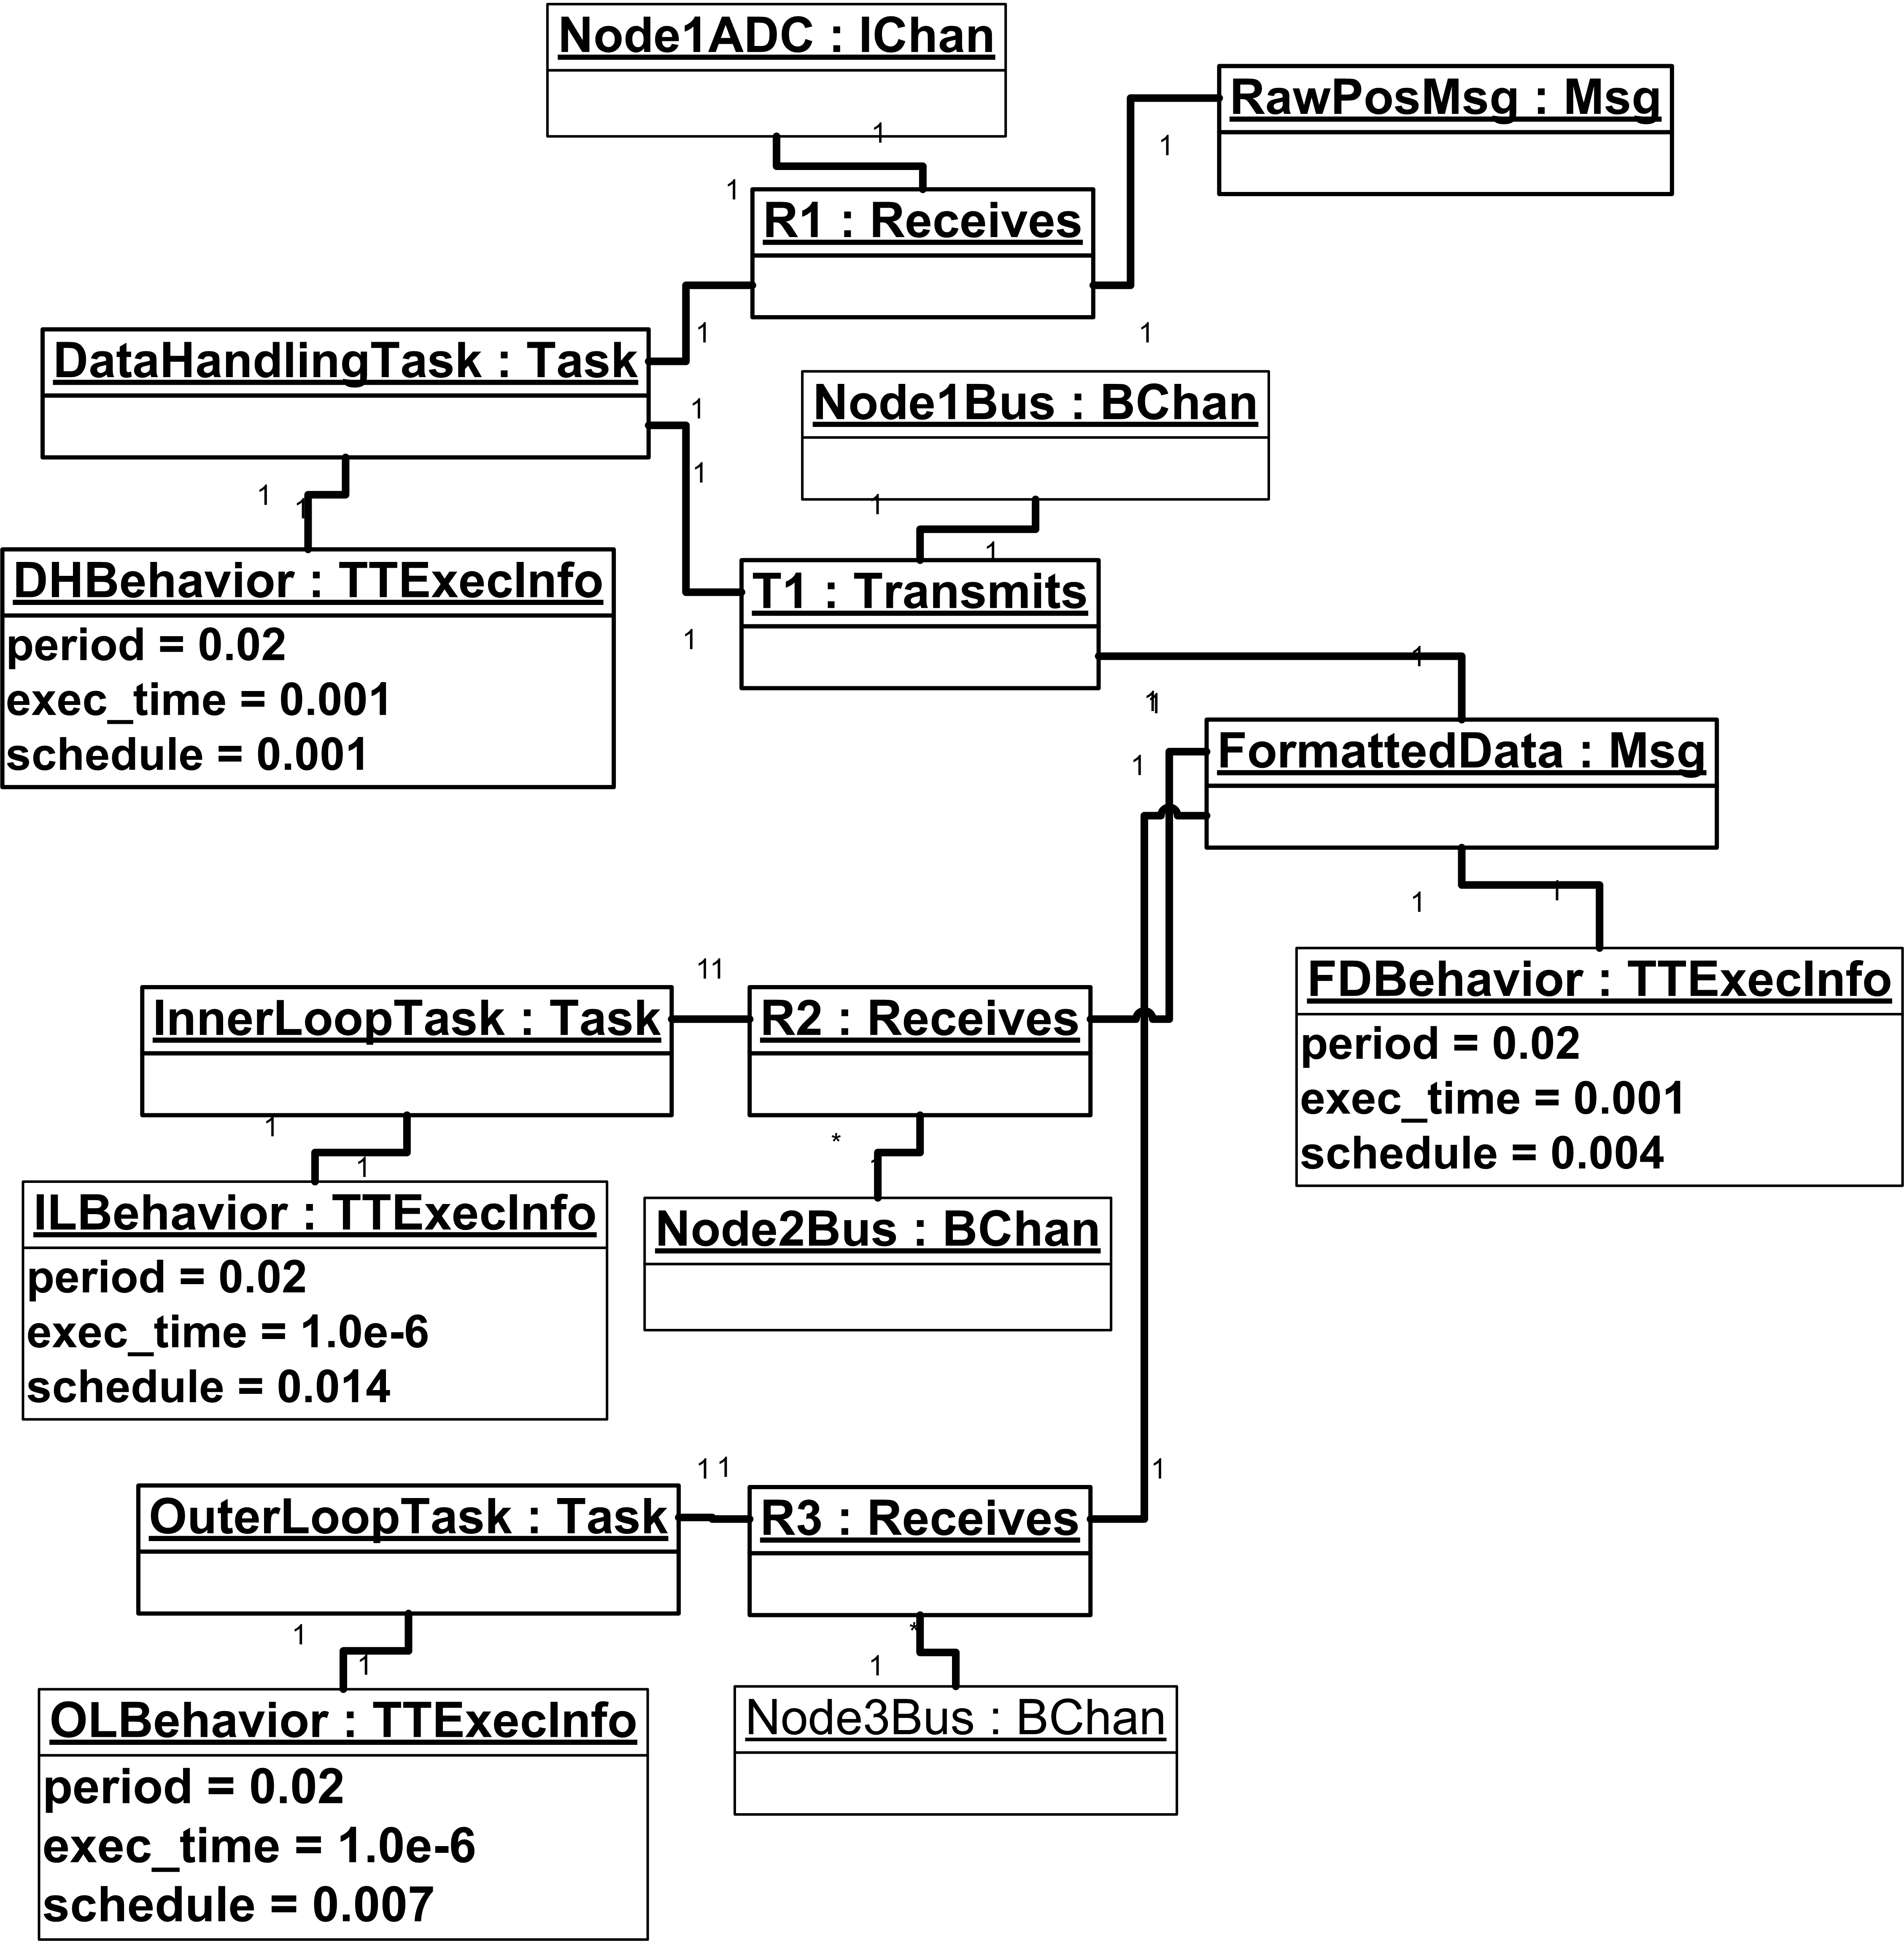
\includegraphics[width=0.87\columnwidth]{figures/msg_struct.png}
    \caption{Abstract semantic model of the message structure from Figs.
\ref{fig:qr_log_arch} and \ref{fig:qr_hw_mapping}. Object diagram showing relation 
objects of type "`Transmits"' and "`Receives"' associate message objects (and their associated behavior objects) 
to sending and receiving tasks, and to node-specific communication channel configurations used to transmit the 
message.  This relation allows us to assemble behavioral information provided by the tasks, messages, and 
platform into a single model.  The schedule interpreter uses information from all of these semantic elements to 
create input for the schedule solver. }
    \label{fig:msg_sched}
\end{figure}
